\documentclass{article}
\usepackage{amsmath}
\usepackage[utf8]{inputenc}
\usepackage{listings}
\usepackage{graphicx}

\graphicspath{ {../results/} }

\lstset{
	basicstyle=\footnotesize,
	numbers=left,
	tabsize=3,
	title=\lstname,
	breaklines=true
}

\addtolength{\oddsidemargin}{-.875in}
\addtolength{\evensidemargin}{-.875in}
\addtolength{\textwidth}{1.75in}

\addtolength{\topmargin}{-.875in}
\addtolength{\textheight}{1.75in}

\title{Lernverfahren autonomer Roboter - Übung 11}
\author{G10\\ Andre Osse\\ Waldemar Stockmann\\ Markus Strehling\\ Tobias Hahn}	
	
\begin{document}
\maketitle
\newpage
\section{Convolutional Neural Networks}

\subsection{Softmax activation function and Cross entropy error}
Beide Funktionen wurden in tools.py wie gewünscht implementiert. Die entsprechenden Codeausschnitte sind im folgenden wiedergegeben, gefolgt von der Konsolenausgabe für den Test:

\subsubsection{Code}
\begin{lstlisting}[caption=Softmax]
def softmax(A):
    A = np.exp(A - np.amax(A, axis=1, keepdims=True))
    return A / np.sum(A, axis=1, keepdims=True)
\end{lstlisting}

\begin{lstlisting}[caption=Cross entropy error]
# Compute error of the dataset
if self.error\_function == "ce":
	return -np.sum(np.log(self.predict(X)) * T)
\end{lstlisting}

\subsection{Output}
\begin{lstlisting}[caption=MLNN Classification Test Output]
Fully connected layer (20 nodes, 20 x 11 weights)
Fully connected layer (10 nodes, 10 x 21 weights)
Fully connected layer (3 nodes, 3 x 11 weights)
Checking gradients up to 6 positions after decimal point...
OK
\end{lstlisting}

\subsection{Convolutional Layer}
Der Convolutional Layer wurde mit Numba implementiert. Die relevanten Codestellen sind angegeben, gemeinsam mit der Ausgabe des Tests.

\subsubsection{Code}
\begin{lstlisting}[caption=Convolve]
for n in range(N):
	for j in range(J):
		for y_o in range(Y_o):
                    for x_o in range(X_o):
                        for i in range(I):
                            for y_k in range(Y_k):
                                for x_k in range(X_k):
                                    A[n,j,y_o,x_o] += kernels[j,i,y_k,x_k] * feature_maps[n,i,y_o*stride_y+y_k, x_o*stride_x+x_k]
                            A[n,j,y_o,x_o] += bias[j,i]
\end{lstlisting}

\begin{lstlisting}[caption=Output Convolutional Test]
Convolutional layer (2 x 8 x 8 nodes, 2 x 1 x 3 x 3 weights)
Convolutional layer (2 x 6 x 6 nodes, 2 x 2 x 3 x 3 weights)
Convolutional layer (2 x 4 x 4 nodes, 2 x 2 x 3 x 3 weights)
Fully connected layer (10 nodes, 10 x 33 weights)
Fully connected layer (2 nodes, 2 x 11 weights)
Checking gradients up to 6 positions after decimal point...Max error: 1.0920861268457293e-08
OK
\end{lstlisting}

\subsection{Connection calculations}
\subsubsection{Input to First Convolutional}
\paragraph{Pixel}
Alle Pixelanzahlen sind immer berechnet auf ein Bild.
Anzahl der Pixel in den Featuremaps: Ein Featurelayer hat $((Original_x - Kernel_x div 2) / Stride_x)) * ((Original_y - Kernel_y div 2) / Stride_y) = 144$.
Von diesen Feauturelayers gibt es 6, also ist die Gesamtpixelanzahl $144 * 6 = 864$.
\paragraph{Connections}
Eine Verbindung sei zwischen zwei Pixeln dann gegeben, wenn der erste Pixel mit seinem Wert Einfluss auf den zweiten Pixel nimmt.
Dann haben die Pixel, die mindestens 9 Pixel Abstand von jedem Rand haben, eine Verbindung mit $3*3 = 9$ Pixel in eine Featuremap, Pixel die weniger Abstand haben $(Abstand_X div 3 + 1) * (Abstand_Y div 3 + 1)$.  Damit ergeben sich bei $28*28$ Pixel Ausgangsbild und 6 Featuremaps $2702 * 6 = 16212$ Verbindungen.
\paragraph{Weights}
Für jede Featuremap gibt es im Layer einen Kernel, der für jeden Pixel Gewichte hat. In den Convolutional Layers hat der Kernel jeweils 25 Pixel, das multipliziert mit 6 ergibt 150 Gewichte für den ersten Layer.

\subsubsection{First Convolutional to second Convolutional}
\paragraph{Pixel}
Anzahl der Pixel in den Featuremaps: Eine Featuremap hat $((Original_x - Kernel_x div 2) / Stride_x)) * ((Original_y - Kernel_y div 2) / Stride_y) = 16$ Pixel.
Von diesen Feauturelayers gibt es 50, also ist die Gesamtpixelanzahl $16 * 50 = 800$.
\paragraph{Verbindungen}
Die Rechnung ist die selbe von oben, allerdings ist es nun so dass die Verbindungen nun nicht mehr von einem Ausgangsbild gerechnet werden sondern von jeder der Featuremaps. Die Berechnung für ein Pixel in einer Featuremap ist noch die gleiche, da sich die Größe des Kernels nicht geändert hat. Jedoch muss diese Pixelanzahl nun mal die Anzahl der Ausgangsfeaturemaps und die Anzahl der Eingangsfeaturemaps gerechnet werden. Damit ergibt sich $242 * 6 * 50 = 72600$.
\paragraph{Weights}
Für jede jede Ausgangsfeaturemap gibt es einen Kernel, dessen Pixel immer Gewichte sind. Damit ergibt sich für diesen Layer mit 50 Featuremaps folgende Gewichtsanzahl $25 * 50 = 1250$ Gewichte.

\subsubsection{Second Convolutional to Last (Fully Connected) Layer}
\paragraph{Verbindungen}
Jeder Pixel in den letzten Featuremaps ist verbunden mit jedem Neuron im Layer. Damit ergibt sich folgende Anzahl der Verbindungen: $800 * 100 = 80000$.
\paragraph{Gewichte}
Die Anzahl der Gewichte ist gleich der Anzahl der Verbindungen, da jede Verbindung ein eigenes Gewicht hat.

\subsubsection{Fully connected layer}
Sei jedes Pixel in den feature maps der Layer ein Neuron, dann gibt es in jedem Layer des Fully Connected Net so viele Verbindungen, die jeweils einem Gewicht entsprechen:
\paragraph{Eingabe zu erstem Hidden Layer}
$28 * 28 * 864 = 677376$ Verbindungen
\paragraph{Erster Hidden zu zweitem Hidden}
$864 * 800 = 691200$ Verbindungen
\paragraph{Zweiter Hidden zu Letztem Hidden}
$800 * 100 = 80000$ Verbindungen
\paragraph{Insgesamt}
Insgesamt wäre die Anzahl der Verbindungen: $677376 + 691200 + 80000 = 1448576$

\subsection{Training CNN}
Das Netzwerk wurde mit den vorgegebenen Parametern trainiert. Die relevante Codestelle dafür ist unten aufgeführt, anschließend die Accuracy und die falsch vorhergesagten Ziffern.

\subsubsection{Code}
\begin{lstlisting}[title=Train CVNN]
    ############################################################################
    # Here you should define and train 'mlnn' (type: MultilayerNeuralNetwork)
    layers = \
        [
            {
                "type": "convolutional",
                "num_feature_maps": 6,
                "kernel_shape": (5, 5),
                "strides": (2, 2)
            },
            {
                "type": "convolutional",
                "num_feature_maps": 50,
                "kernel_shape": (5, 5),
                "strides": (2, 2)
            },
            {
                "type": "fully_connected",
                "num_nodes": 100
            }
        ]
    
    mlnn = MultilayerNeuralNetwork(
        D=(1, 28,28), F=10, layers=layers, std_dev=0.01,
        verbose=1)
    mbsgd = MiniBatchSGD(net=mlnn, epochs=15, batch_size=32, alpha=0.01, alpha_decay=0.9999, min_alpha=0.00005, eta=0.5, eta_inc=0.00001, max_eta=0.9, random_state=0, verbose=1)
    mbsgd.fit(train_images, train_targets)

    ############################################################################
\end{lstlisting}

\lstinputlisting{../code/error.py}

\subsubsection{Output}
\begin{lstlisting}[title=Console Output]
Accuracy on test set: 98.76 %
Error = 476.353
\end{lstlisting}

\subsubsection{Results}
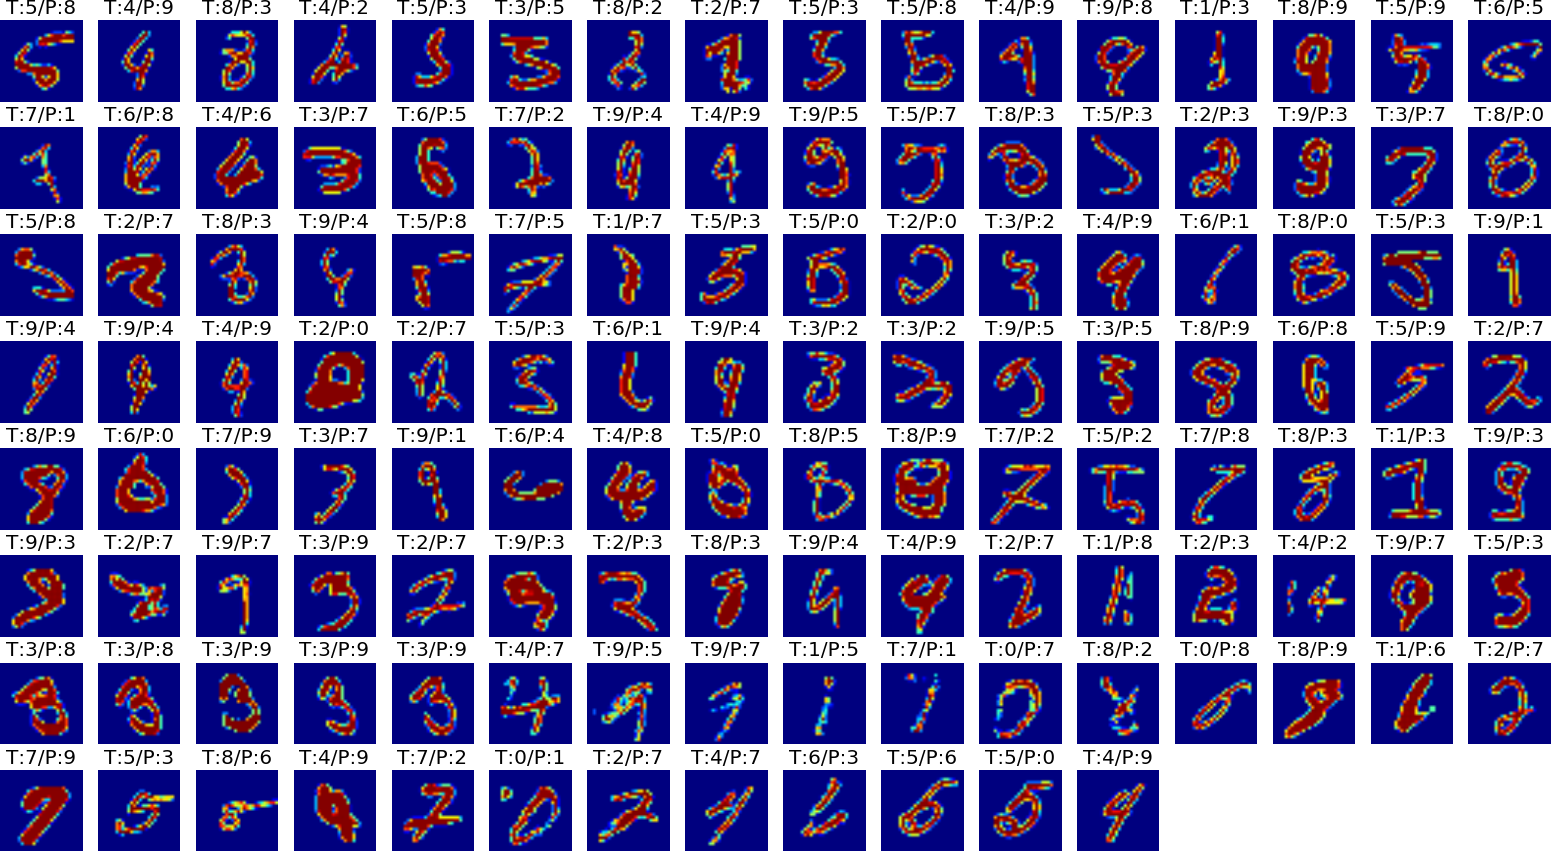
\includegraphics[width=\textwidth]{mnist.png}

\end{document}
